\begin{figure}[htp]
  \centering
  \begin{subfigure}[b]{0.45\textwidth}
    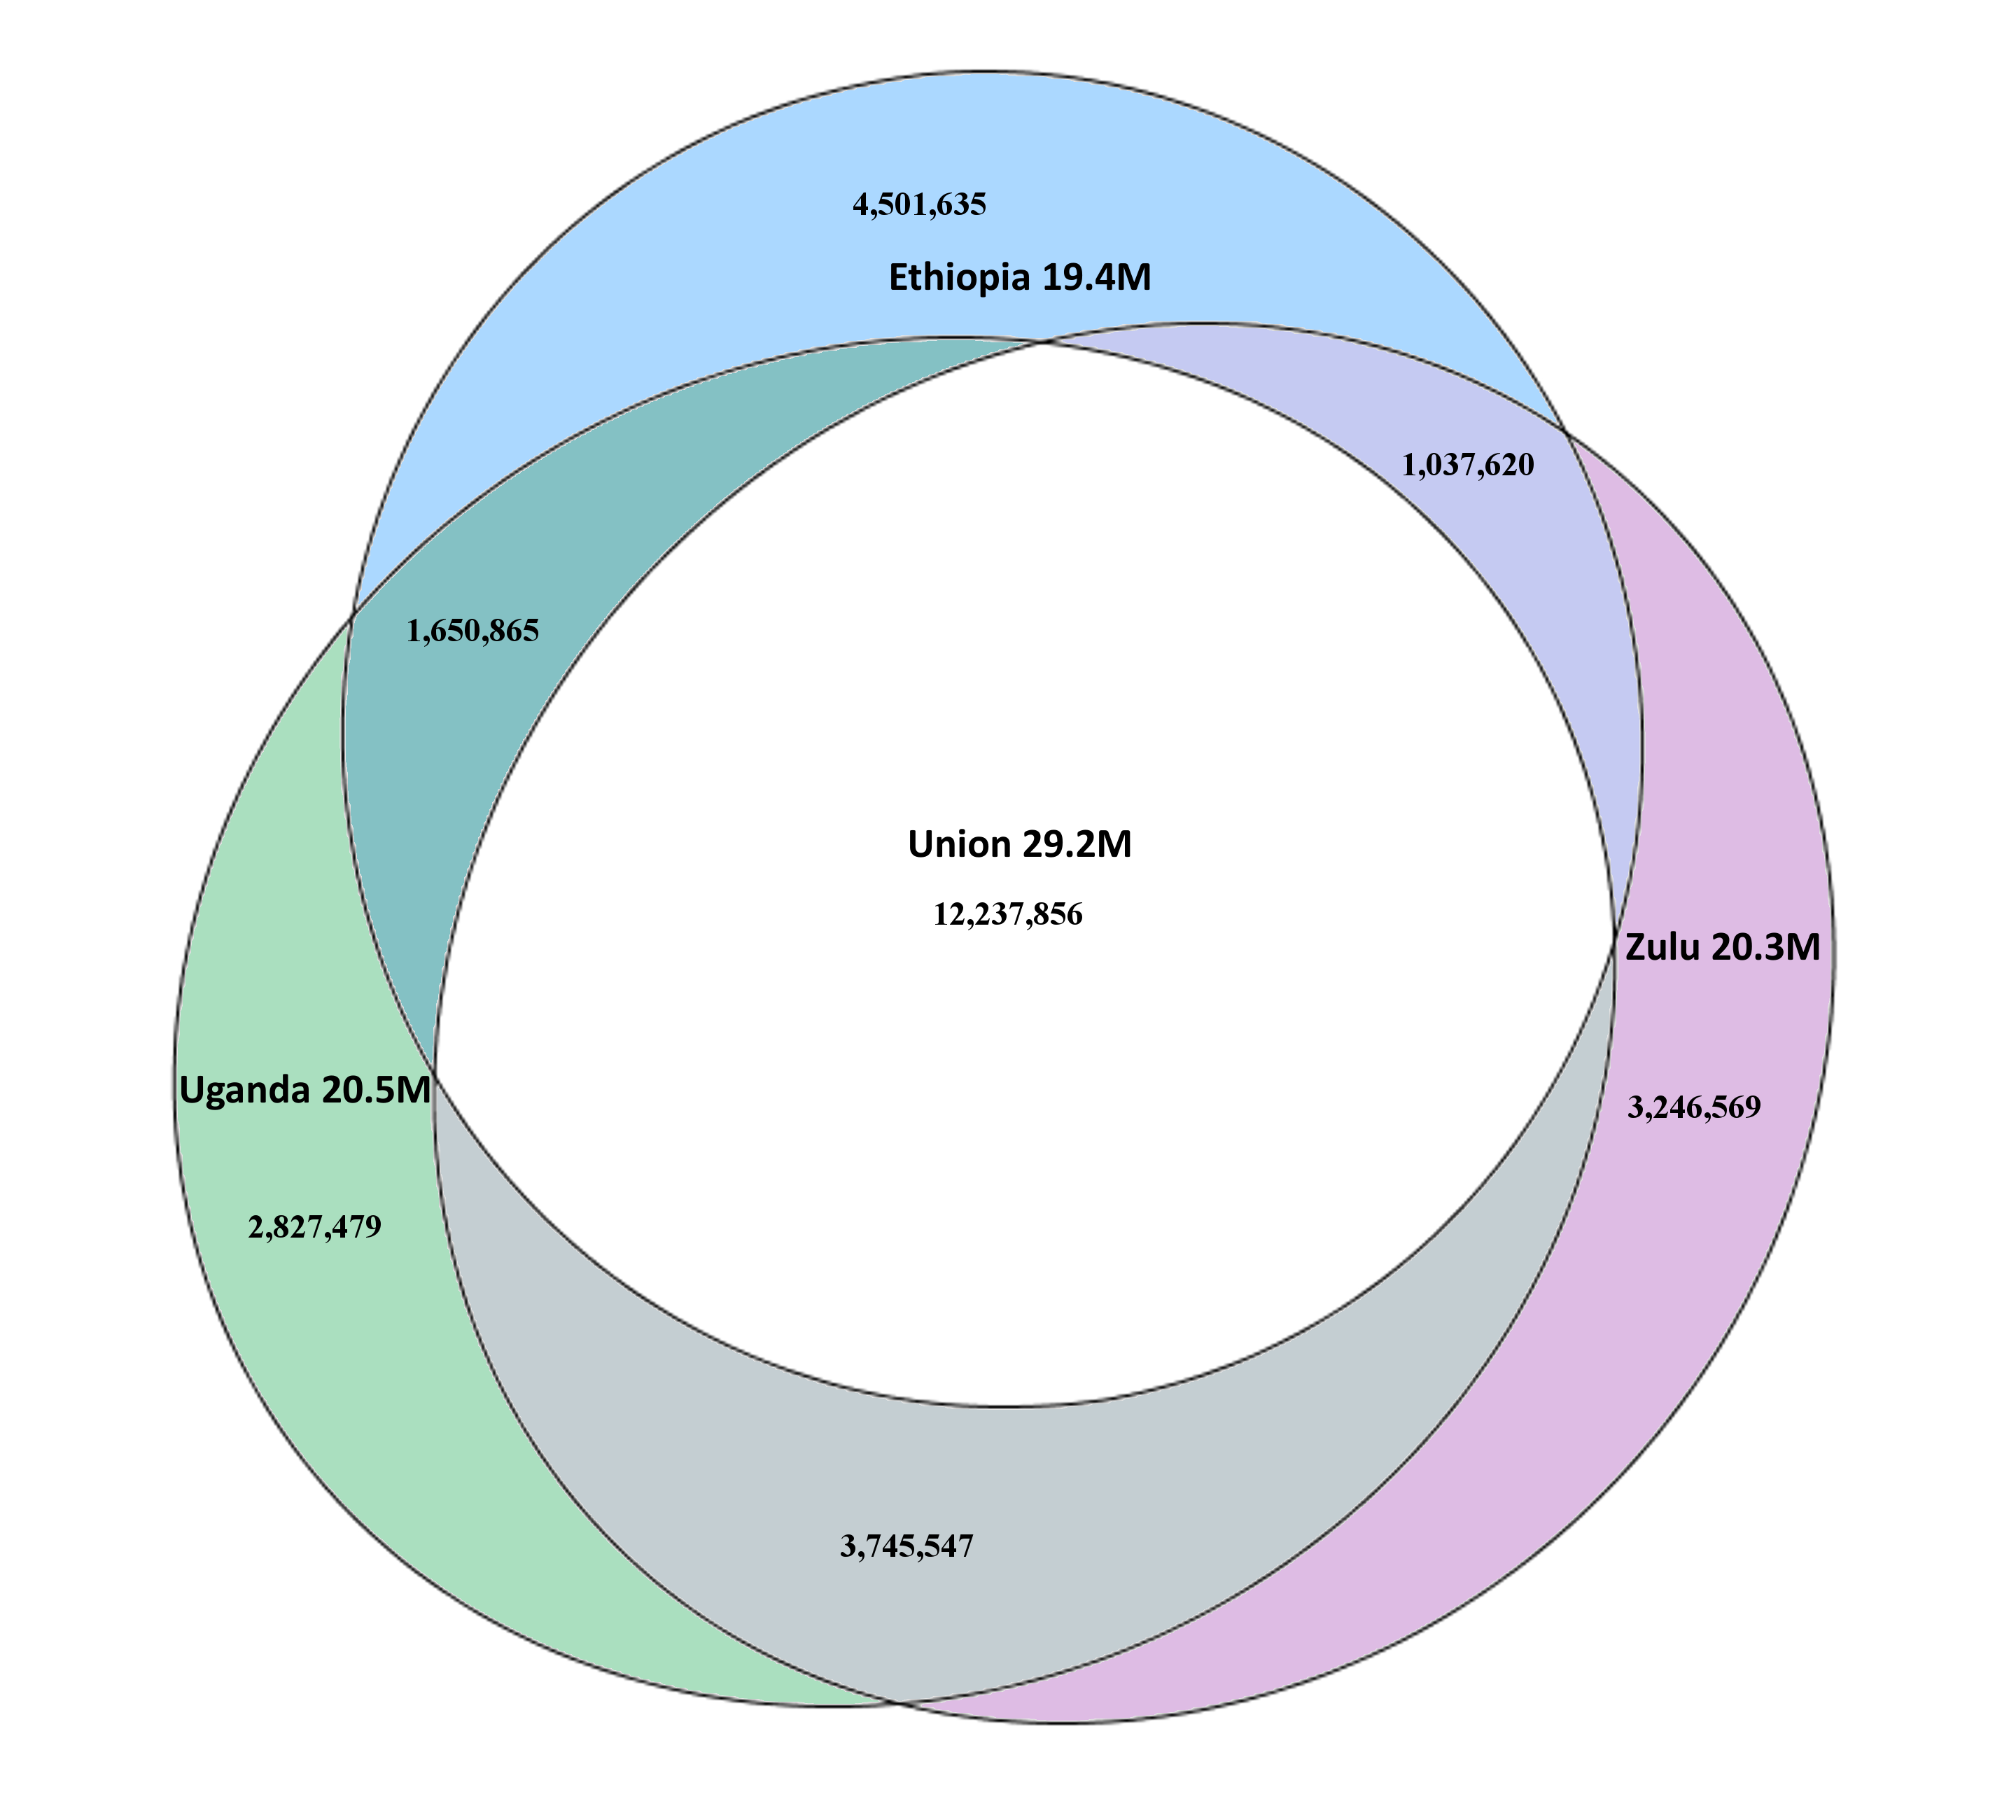
\includegraphics[width=\textwidth]{fig/venn3.png}
    \caption{}
  \end{subfigure}
  \begin{subfigure}[b]{0.45\textwidth}
    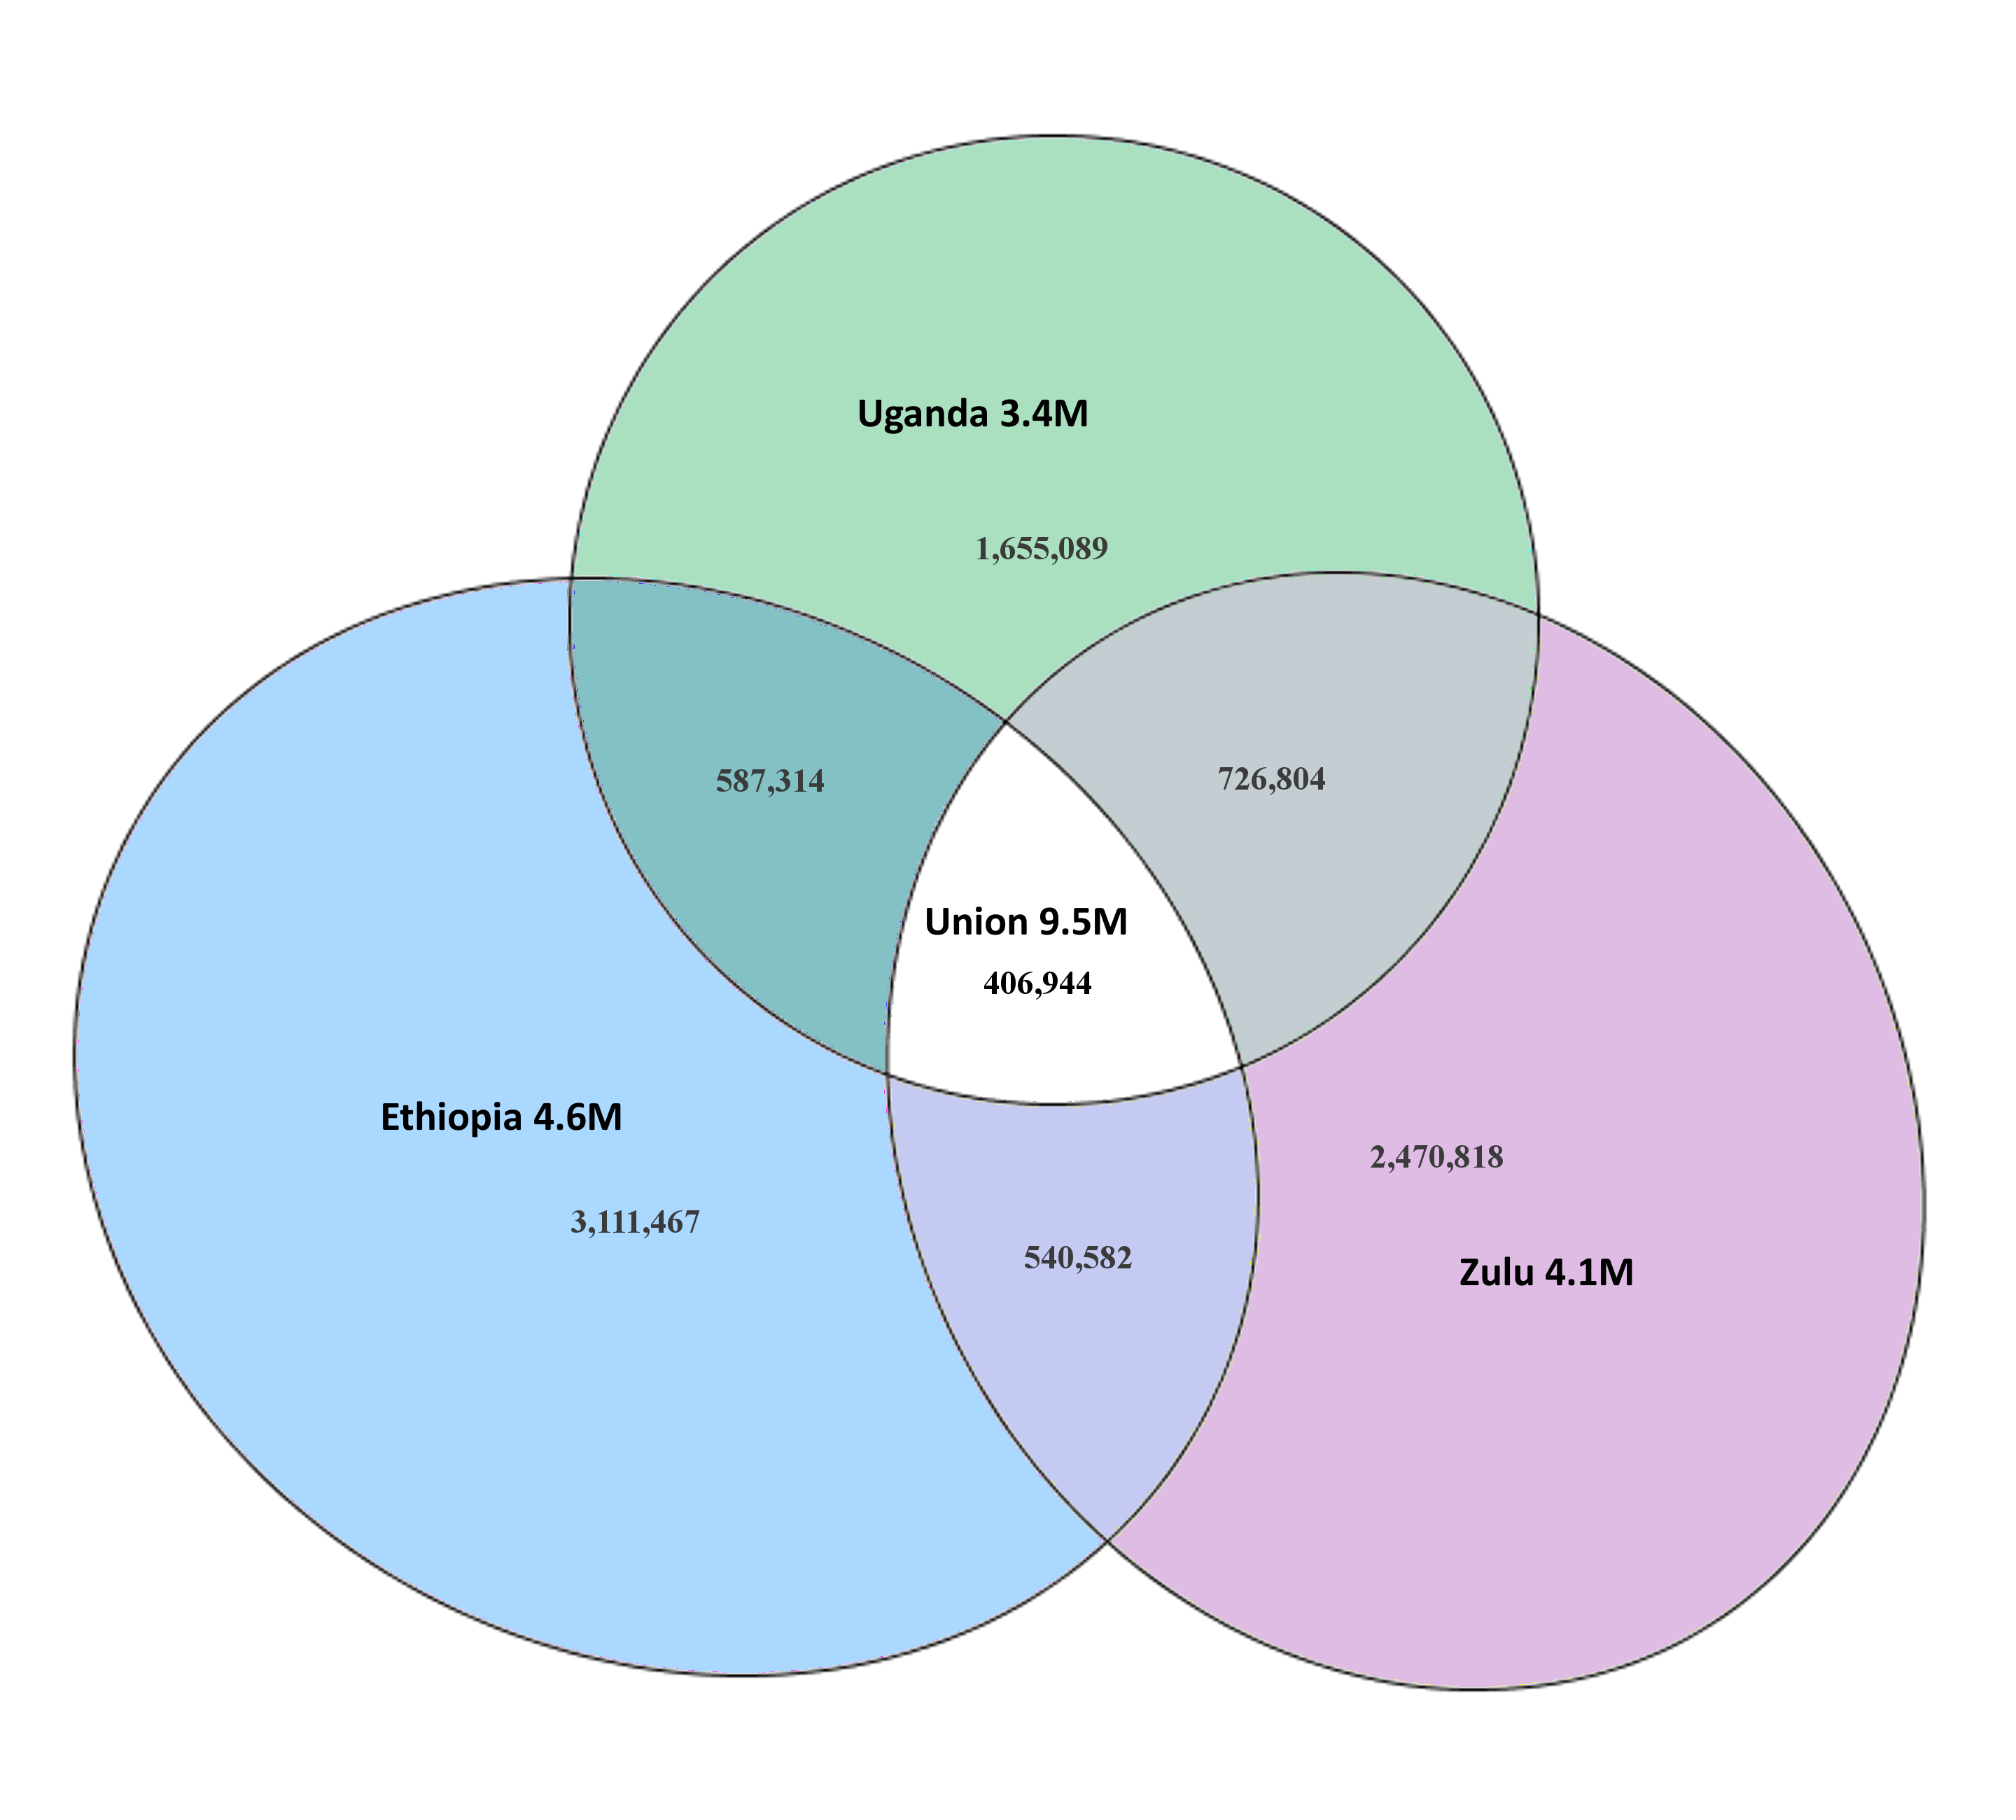
\includegraphics[width=\textwidth]{fig/venn3_complement.png}
    \caption{}
  \end{subfigure}
  \begin{subfigure}[b]{0.45\textwidth}
    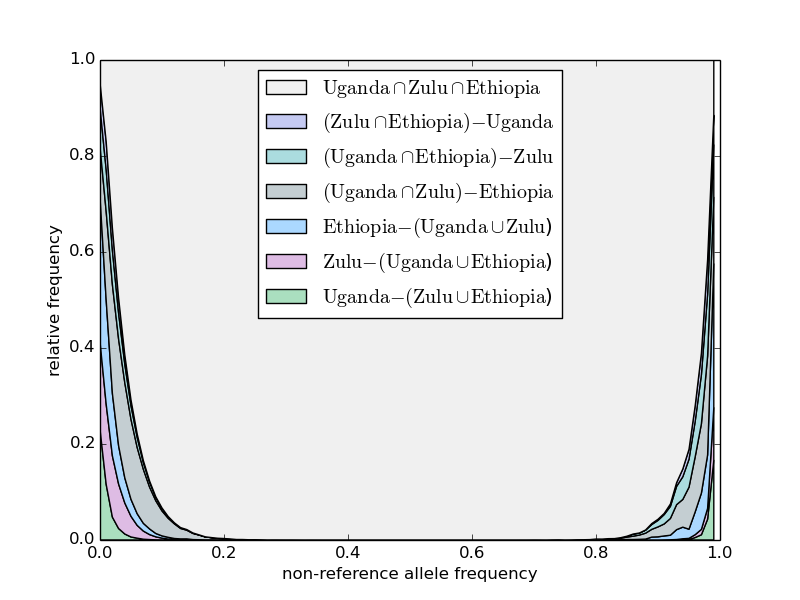
\includegraphics[width=\textwidth]{fig/venn3_stackplot_SNPs.png}
    \caption{}
  \end{subfigure}
  \begin{subfigure}[b]{0.45\textwidth}
    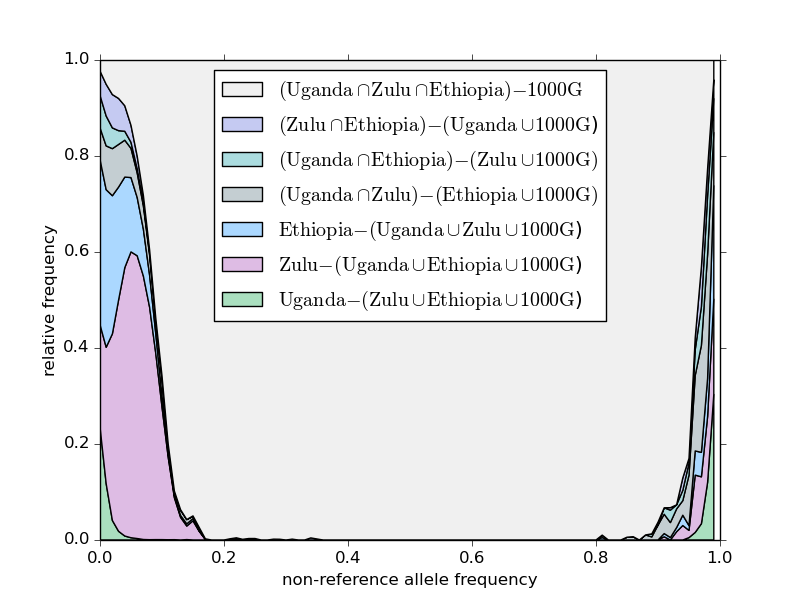
\includegraphics[width=\textwidth]{fig/venn3_stackplot_complement_1000G_SNPs.png}
    \caption{}
  \end{subfigure}
  \caption{Sharing of variants between populations. a) SNP intersection between the 3 sequenced populations subsampled to 100 samples and downsampled to 4x coverage. b) Intersection between the novel variants in the 3 populations; i.e. variants in the relative complement of \gls{1000G} phase 1 with respect to the 3 populations. c) Relative allele frequency spectra for variants in different sets of the Venn diagrams depicted in a and b. The majority of the novel variants with respect to \gls{1000G} are unique to each population. Area proportional Venn diagrams were created with eulerAPE\cite{10.1371/journal.pone.0101717} and stacked plots were created with matplotlib\cite{Hunter2007}}
  \label{fig:intersection}
\end{figure}